\documentclass{article}


%preamble
%required
%\usepackage{Sweave} %Integrates R code with LaTeX for creating dynamic reports
\usepackage{natbib}%Provides citation and bibliography support
\usepackage{amsmath}%Enhances mathematical typesetting capabilities.
\usepackage{textcomp}%among other things, it allows degrees C to be added
\usepackage{float}%Helps with precise figure placement using the [H] option.
\usepackage[utf8]{inputenc} % allow funny letters in citations 
\usepackage[T1]{fontenc}
\usepackage[nottoc]{tocbibind} %should add Re fences to the table of contents?
\usepackage{amsmath} % making nice equations 
\usepackage{listings} % add in stan code
\usepackage{xcolor}
\usepackage{capt-of}%allows me to set a caption for code in appendix 
\usepackage[export]{adjustbox} % adding a box around a map
\usepackage{lineno}
\linenumbers

\usepackage[margin=2cm]{geometry}
\usepackage[most]{tcolorbox}

\newtcolorbox{mytextbox}[1][]{% specify textbox
	sharp corners,
	enhanced,
	colback=white,
	height=15cm,
	attach title to upper,
	#1
}

% recommended! Uncomment the below line and change the path for your computer!
% \SweaveOpts{prefix.string=/Users/Lizzie/Documents/git/teaching/demoSweave/Fig.s/demoFig, eps=FALSE} 
%put your Fig.s in one place! Also, note that here 'Fig.s' is the folder and 'demoFig' is what each 
% Fig. produced will be titled plus its number or label (e.g., demoFig-nqpbetter.pdf')
% make your captioning look better
\usepackage[small]{caption}

\usepackage{xr-hyper} %refer to Fig.s in another document
\usepackage{hyperref}

\setlength{\captionmargin}{30pt}
\setlength{\abovecaptionskip}{0pt}
\setlength{\belowcaptionskip}{10pt}

% optional: muck with spacing
\topmargin -1.5cm        
\oddsidemargin 0.5cm   
\evensidemargin 0.5cm  % same as odd side margin but for left-hand pages
\textwidth 15.59cm
\textheight 21.94cm 
% \renewcommand{\baselinestretch}{1.5} % 1.5 lines between lines
\parindent 0pt		  % sets leading space for paragraphs
% optional: cute, fancy headers
\usepackage{fancyhdr}
\pagestyle{fancy}
%\fancyhead[LO]{Frederik Baumgarten}
%\fancyhead[RO]{Research Proposal}
% more optionals! %

\usepackage{graphicx}
\graphicspath{{/Users/frederik/github/PlantDeterminism/figures/}} % specify the path to your figures directory




\begin{document}
	
	
	\title{Invest now, get paid later? Limits and opportunities of woody plants to time growth in a future climate %(my favourite)
		
		%dlDec18: Alternate title ideas:
		%Growth determinism/determinacy/habits in plants/woody perennials/trees: Limits and opportunities to time growth in a future climate. 
		
		%Growth determinacy in temperate trees: investing at the right time to cope with environmental stress and benefit from extended growing seasons in a future climate.
		
		%Invest now, get paid later? Growth strategies to cope with environmental stress and benefit from extended growing seasons in a future climate
		
	
	} 
	
	\date{\today}
	\author{Frederik Baumgarten\textsuperscript{1-3}, Sally Aitken\textsuperscript{1}, Yann Vitasse\textsuperscript{3}, Robert D Guy\textsuperscript{1}, EM Wolkovich\textsuperscript{1}}
	\maketitle
	
	$^1$ Department of Forest and Conservation, Faculty of Forestry, University of British Columbia, 2424 Main Mall
	Vancouver, BC Canada V6T 1Z4. \\
	
	$^2$  
	Department of Environmental Sciences-Botany, University of Basel, Schönbeinstrasse 6, Basel 4056, Switzerland. \\
	
	$^3$  
	Swiss Federal Institute for Forest, Snow and Landscape Research WSL, Zürcherstrasse. 111, Birmensdorf 8903, Switzerland
	\\
	
	Corresponding Author: Frederik Baumgarten; frederik.baumgarten@unibas.ch \\
	Journal: Perspective in Ecology Letters
	
	%Full word count: \\
	%Summary word count: \\
	%Introduction word count: \\
	%Materials and Methods word count: \\
	%Results and figure legends word count: \\
	%Discussion word count: \\
	
	%werwolve: how is tree growth impacted by climate change? 1) by extreme events and 2) by an extended growing season? 
	%baby: better predictions of when environmental factors are influencing growth taking into account the phenological sequence of a species
	%silverbullet: concept of determinism
	
	
\section*{Abstract} %200 words for perspective 
	When and how much organisms grow given environmental constraints and opportunities are fundamental questions in biology, and especially pressing in the context of climate change as we strive to accurately predict biomass production and carbon sequestration. While environmental factors such as temperature and water availability directly regulate plant growth, the timing and rate of growth is also governed by a plant’s phenological sequence—its genetically programmed developmental stages. This sequence is critical for predicting climate responses but is often overlooked.
	
	Here, we leverage the concept of (in-)determinacy in growth and development—which captures how flexibly plants produce new organs from preformed cells versus initiating them \textit{de novo}—to propose a new framework for predicting tree growth responses to climate change.
	
	We hypothesize that: 1) determinate growth is an adaptation to predictable seasonal climates, restricting new tissue investment to a short favorable period before dormancy; 2) indeterminate species may recover more effectively from damage, giving them an advantage under increasing climatic extremes; and 3) species with higher indeterminacy are more likely to benefit from lengthening frost-free growing seasons. 
	We argue that future carbon sequestration may depend not only on how environmental factors change, but also on the degree of determinacy set by a species’ intrinsic genetic programming.\\
		% : the ability of trees to preform tissue as an investment for next year’s growth that will overwinter in buds vs. a strategy that additionally relies on the continuous activity of the apical meristem throughout the growing season (neo-formed tissue)
		
			\textbf{Keywords}: plant growth, tree phenology, shoot extension, indeterminate growers, carbon sequestration, growing season length, drought, genetic programming, phenotypic plasticity, forest productivity
			\newpage
			
\section*{Introduction}
		Investing the right amount of resources in growth at the right time is of crucial importance to the survival and fitness of any living organism. The topic of growth strategies and habits has a long history in science, spanning the fields of genetics, genomics, physiology and ecology across the animal and plant kingdoms \citep{stearnsEvolutionLifeHistories1998a}. At its core lies the concept of determinacy—the classification of organisms as either reaching a fixed size at maturity or continuing to grow throughout their lives. Like mollusks, fish and reptiles, plants add to their primary bodies as long as they live and are therefore considered ‘indeterminate growers’  \citep{ejsmondHowTimeGrowth2010}. Various terms have emerged to describe this phenomenon across spatial and temporal scales, e.g. from a single cell to the whole organism, and from a single season to an entire lifetime \citep{mcdanielInductionDeterminationDevelopmental1992a, karkachTrajectoriesModelsIndividual2006}. In plants, organs can develop from preformed embryonic tissue (e.g. primordia in overwintering buds), form \textit{de novo}, or both, depending on species. Yet, it remains unclear which point along this trait continuum will prove more advantageous in a future climate characterized by increased environmental stress and prolonged growing seasons. In the following we briefly outline the fundamental limitations to plant growth in extra-tropical regions by linking external environmental drivers and internal growth control mechanisms to introduce a framework for predicting when and how much trees and other woody plants in general may grow and discuss their role in a future climate. \\
		
		% In some tropical ecosystems a continued production of tissue by trees can be both possible and advantageous; in all other regions, however, strategies that rely on growth from stored reserves and pre-built tissue are common.

	\subsection*{Seasonality of temperature, soil moisture and light}
		The further one travels from the equator towards the poles, the more strongly plants are confined to a shrinking time window of opportunity set primarily by low temperatures. Below c. 5 °C, metabolic activity slows to an extent where growth and development largely cease \citep{schenkerPhysiologicalMinimumTemperatures2014, rossiCriticalTemperaturesXylogenesis2008, kornerWinterCropGrowth2008}. More importantly, sub-freezing temperatures can cause severe damage to plant tissue if they occur at vulnerable developmental stages, e.g. during or after leaf unfolding, prior to fruit maturation, or before cold acclimation in fall \citep{sakaiFreezingInjuriesPlants1987c, baumgartenNoRiskNo2023a}. 
		While annual plant species accommodate their entire life cycle within this window, perennial plants are forced to partition their growing phase seasonally, with periods of activity alternating with periods of dormancy. This is referred to as intermittent or rhythmic (as opposed to continuous) growth. \\

		During the active growing season, high temperatures can also directly inhibit growth and development, by surpassing species-specific physiological thresholds \citep{osullivanThermalLimitsLeaf2017}. Indirectly, high temperatures often reduce soil moisture, leading to water stress that can slow or stall growth \citep{hsiaoPlantResponsesWater1973, pugnaireConstraintsWaterStress1999, etzoldNumberGrowthDays2021}, and in extreme cases, cause leaf scorching or premature senescence \citep{estiarteAlterationPhenologyLeaf2015a}. Together, these temperature and soil moisture limitations act as environmental filters, narrowing the period during which growth is possible (Figure \ref{fig:fig_1xxx}).  \\
		
		Light also influences plant growth through two key processes. First, light is the basic energy source (light intensity and quality) driving photosynthesis and consequently source activity. Second, the length of the daily periods of light and dark (photoperiod), mediate many physiological processes including bud set and dormancy transitions \citep{wangPlantsDistinguishDifferent2024b}. Both factors may contribute to the common observation that plant growth often peaks near the summer solstice in extra-tropical regions \citep{rossiConifersColdEnvironments2006, etzoldNumberGrowthDays2021, luoSummerSolsticeMarks2018} or that a window of temperature sensitivity 'opens’ around the summer solstice to synchronize reproductive efforts over very large spatial scales \citep{journeSummerSolsticeOrchestrates2024}.
		
		\subsection*{Internal programming of plants}
		Given our relatively robust understanding of environmental influences on plant growth, it may seem straightforward to predict tree growth under current and future climatic conditions. Yet, this proves challenging, particularly when predicting responses under scenarios with extended, climatically favorable growing seasons \citep{zohnerHowChangesSpring2021}. Here we propose that accurate predictions require incorporating another key, but often overlooked, factor: internal growth control---the genetically encoded developmental program that may prevent further growth \textit{despite} favorable environmental conditions.\\
		
		While plants have evolved numerous morphological adaptations to tolerate or avoid harmful environmental conditions, most temperate and boreal species cope with predictable seasonal fluctuations in temperature and moisture by temporally escaping these conditions. They do this by aligning their life-history events (phenology) with a cycle of growth and dormancy that balances survival, reproduction, and growth over the long lifespan typical of many tree species. Hence, the phenological sequence can impose abrupt internal switches in resource allocation---from vegetative growth to reproduction (flowering, fruit maturation) and storage \citep{stearnsTradeOffsLifeHistoryEvolution1989, chapinEcologyEconomicsStorage1990}. These transitions act as additional internal filters, further narrowing the effective window during which vegetative growth can occur, regardless of environmental potential (Figure \ref{fig:fig_1xxx}).\\
		
		\subsection*{Aim of this perspective/Growth responses in future climates}% any better idea?
		Climate change is extending the length of the growing season while simultaneously increasing the frequency and severity of environmental stressors such as drought \citep{haoChangesSeverityCompound2018} and presumably also late spring frost events in many regions worldwide \citep{zohnerLatespringFrostRisk2020}. How are these potential opportunities and threats linked to species-specific growth performance? To what extent do growth responses depend on the strategy to either preform and/or initiate new shoot tissue \textit{de novo} in the current growing season (i.e., its degree of determinacy; see next section)? Which strategy profits most from an extended growing season length and which one can cope better with increased environmental stress? Finally, when might each strategy ultimately be more productive in terms of biomass accumulation and carbon sequestration under a warmer, drier climate?
		
		The role of primary growth has been widely neglected in addressing these questions, even though it affects photosynthetic capacity and therefore biomass production to a large degree \citep{girardPolycyclismFundamentalTree2011}. 
		In this perspective we revisit classical concepts of shoot growth patterns, generalize them across meristem types and position them within the context of climate change. We propose that mechanisms of internal growth control---especially those governing the degree of determinacy---are key features shaping how trees will respond to future climatic conditions.
		
								\begin{figure}
								\centering
								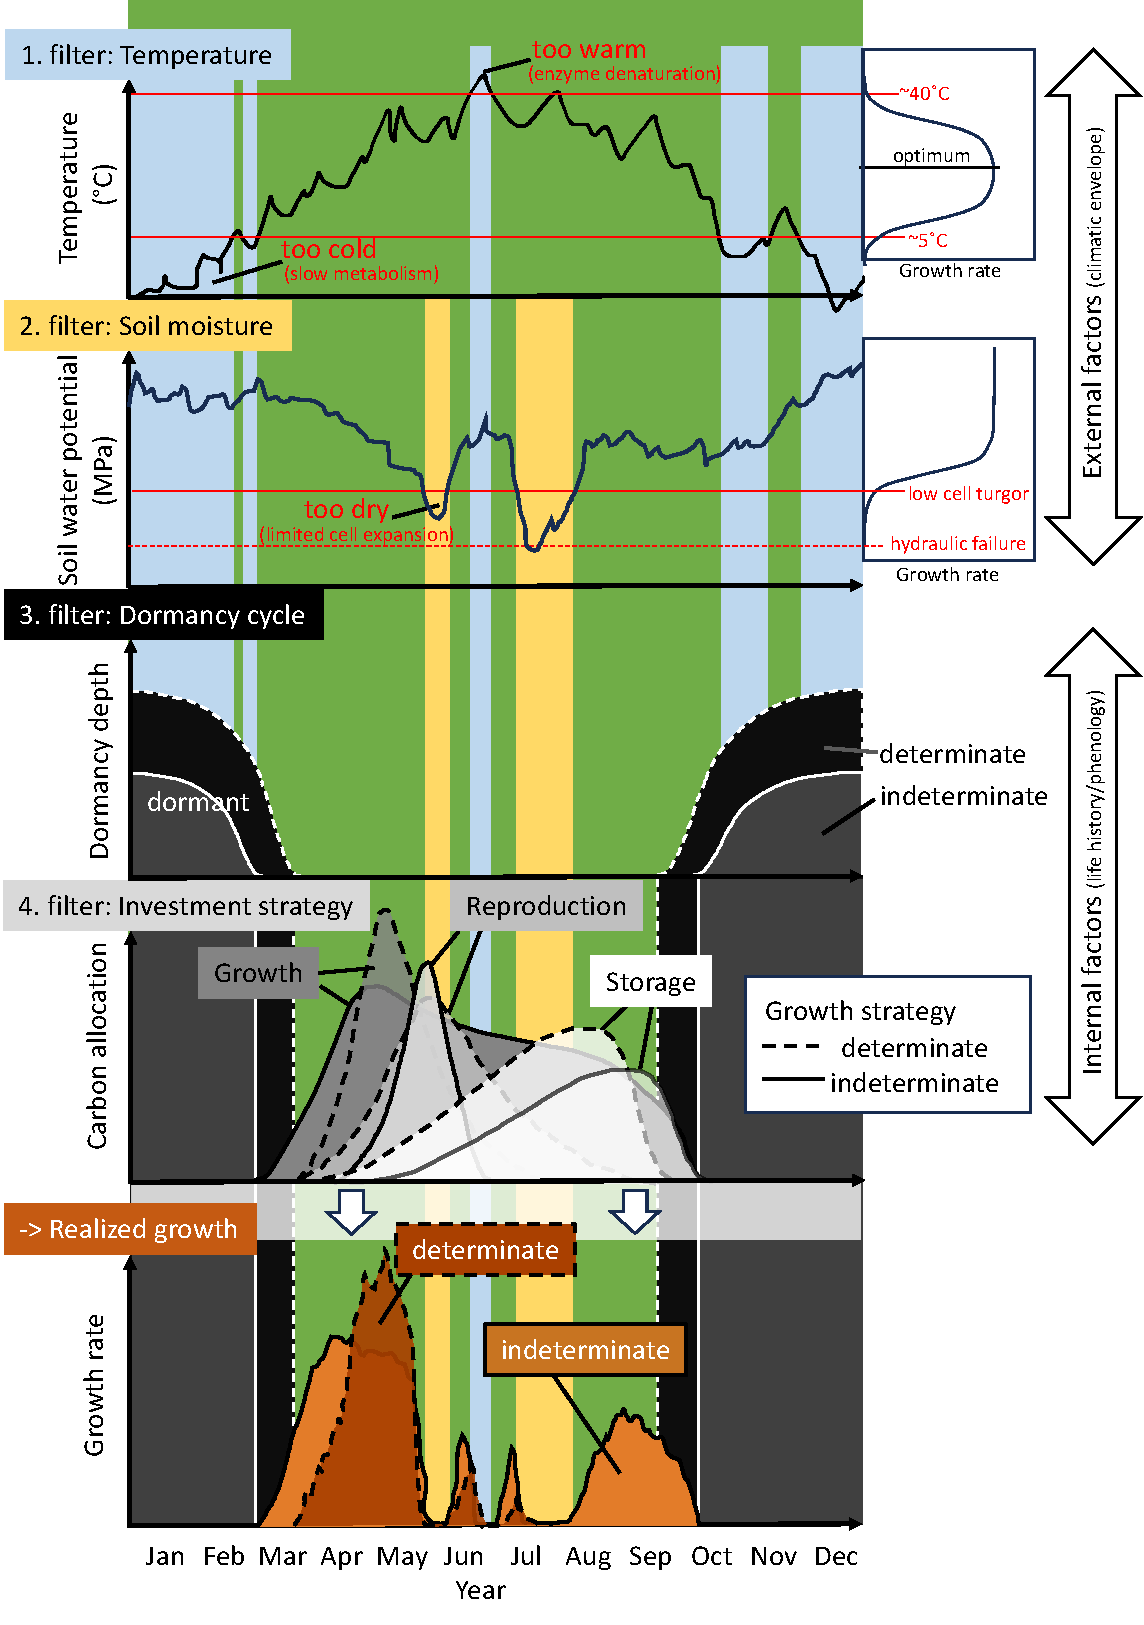
\includegraphics[width=0.9\textwidth]{Fig_1_V6.pdf} 
								\caption{Schematic overview of the possible discrepancy between the potential growing season and the effectively realized vegetative growth. Environmental factors like temperature and soil moisture, exceeding growth-promoting thresholds can be seen as filters that narrow the window of opportunity available for vegetative growth. Potential light and photoperiodic constraints are not shown. The species-specific life history cycle (phenology) can impose another filter by dictating a dormancy cycle and prioritizing developmental processes other than vegetative growth (e.g. flowering, fruit maturation and storage). The degree of (in)determinacy is presented here in two extremes, although we propose to consider this trait as continuous.}
								\label{fig:fig_1xxx}
								\end{figure}
								
\section*{The concept of (in)determinate growth}

	\subsection*{Full stop or temporary break in (vegetative) growth}
	In annual plants, growth ends with the production of flowers to form fruits and seeds: a signal in the apical meristem triggers a sudden switch in resource investment from vegetative growth to building a reproductive structure with no point of return, signaling the end of the life-cycle \citep{poethigPhaseChangeRegulation2003, huijserControlDevelopmentalPhase2011}. A shoot axis that terminates in a flower or other modified structure and ceases meristematic activity is considered `determinate' \citep{barthelemyPlantArchitectureDynamic2007}. In woody perennial species, however, flowers are typically produced on lateral shoots or buds, preserving the main vegetative axis and allowing continued structural expansion. However, `determinate growth' also refers to a temporal suspension of the meristem, which leads to a time lag between the formation of organs and their expansion \citep{kozlowskiSeedGerminationOntogeny2012, halleTropicalTreesForests1978}. 
	
	%yannJuly5: so basically all temperate trees as primordial leaves are formed in the buds before winter. Should we say then that all plants forming buds before the unfavorable season (cold or dry period) are per definition ‘determinate growth’ but the difference occurs during the favorable season where some just expand what has been preformed/planned in the buds, some make new leaves continuously during the growing season after expanding the ones preformed in the buds and some stop after expanding leaves from the buds for a while and make a second flush later (polycyclic growth species)
	
	%robJuly21: To avoid confusion, I think more is needed here to differentiate lateral buds/shoots from terminal buds/shoots, and also to indicate that further discussion mostly relates to the latter.  Even in indeterminate species, most lateral shoots (i.e., the so-called “short” shoots) are determinate whether they hold just leaves or have both leaves and additional tertiary shoots that become flowers.  
	
	%While lateral shoots can be suppressed permanently (so called `short shoots'), terminal shoots commonly follow a such a temporal suspension can be almost permanent in the case of lateral shoots (), 
		
	%Shoot growth patterns do not only tell us something about the plant architecture and the strategy of space exploitation, but may reveal also patterns of the whole-plant dynamic and potential of growth and carbon sequestration.
	
	%unit of extension vs. unit of morphogenesis: Perhaps state somewhere that we commonly only observe the extension pattern while patterns of organogenesis remain hidden. 
	
	%indeterminate growth: functioning of the apical meristems remains intact (but may have periods of rest)
	
	
	\subsection*{When to form (new) tissue}
	In their first year, all seedlings exhibit indeterminate growth. In subsequent years, many temperate and boreal tree species preform their new shoot increments during the previous growing season, overwintering them as primordial shoots with leaves and internodes in hardened buds to be `ready-to-go' when spring arrives. Once the leaves flush and the internodes elongate, some species suppress further activity of the apical meristem for the rest of the season through internal control mechanisms such as paradormancy \citep{langEndoParaEcodormancy1987}, often regulated by photoperiod-induced hormonal changes \citep{bohleniusCOFTRegulatory2006a}. Other species, by contrast, continue to produce neoformed leaves and internodes that build on preformed growth, in some cases stretching their indeterminate growth period into autumn until low temperature forces them to stop. Indeterminate growth can occur either through the continuous activity of the shoot apical meristems forming new leaves and internodes without buds, termed free growth, or through the formation and subsequent flushing of buds mid-season without a period of dormancy, called second flushing or lammas growth (Figure \ref{fig:fig_2xxx}). \\
	As we use it here, (in)determinacy in trees refers to the ability to:\\
	a) preform organs in one year as a future investment, which is deployed rapidly in the following spring with no further primary shoot growth during that season (determinate strategy)\\
	b) maintain a continuous or episodic meristem activity by forming new shoot tissue during the current growing season (indeterminate strategy).\\

Although this concept is often presented dichotomously \citep{kozlowskiGrowthControlWoody1997, lechowiczWhyTemperateDeciduous1984a}, but see \citealp{kikuzawaLeafSurvivalWoody1983, damascosBudCompositionBranching2005}), with species classified as either determinate or indeterminate growers, most species likely exist along a gradient with numerous intermediate forms. For instance, many oaks (\textit{Quercus spp.}) are considered determinate growers, but can exhibit multiple flushes. Similarly, Douglas-fir (\textit{Pseudotsuga menziesii}) gradually adopts a more determinate growth habit with maturity \citep{borchertConceptJuvenilityWoody1976, heuretOntogeneticTrendsMorphological2006}.\\

								\begin{figure}
								\centering
								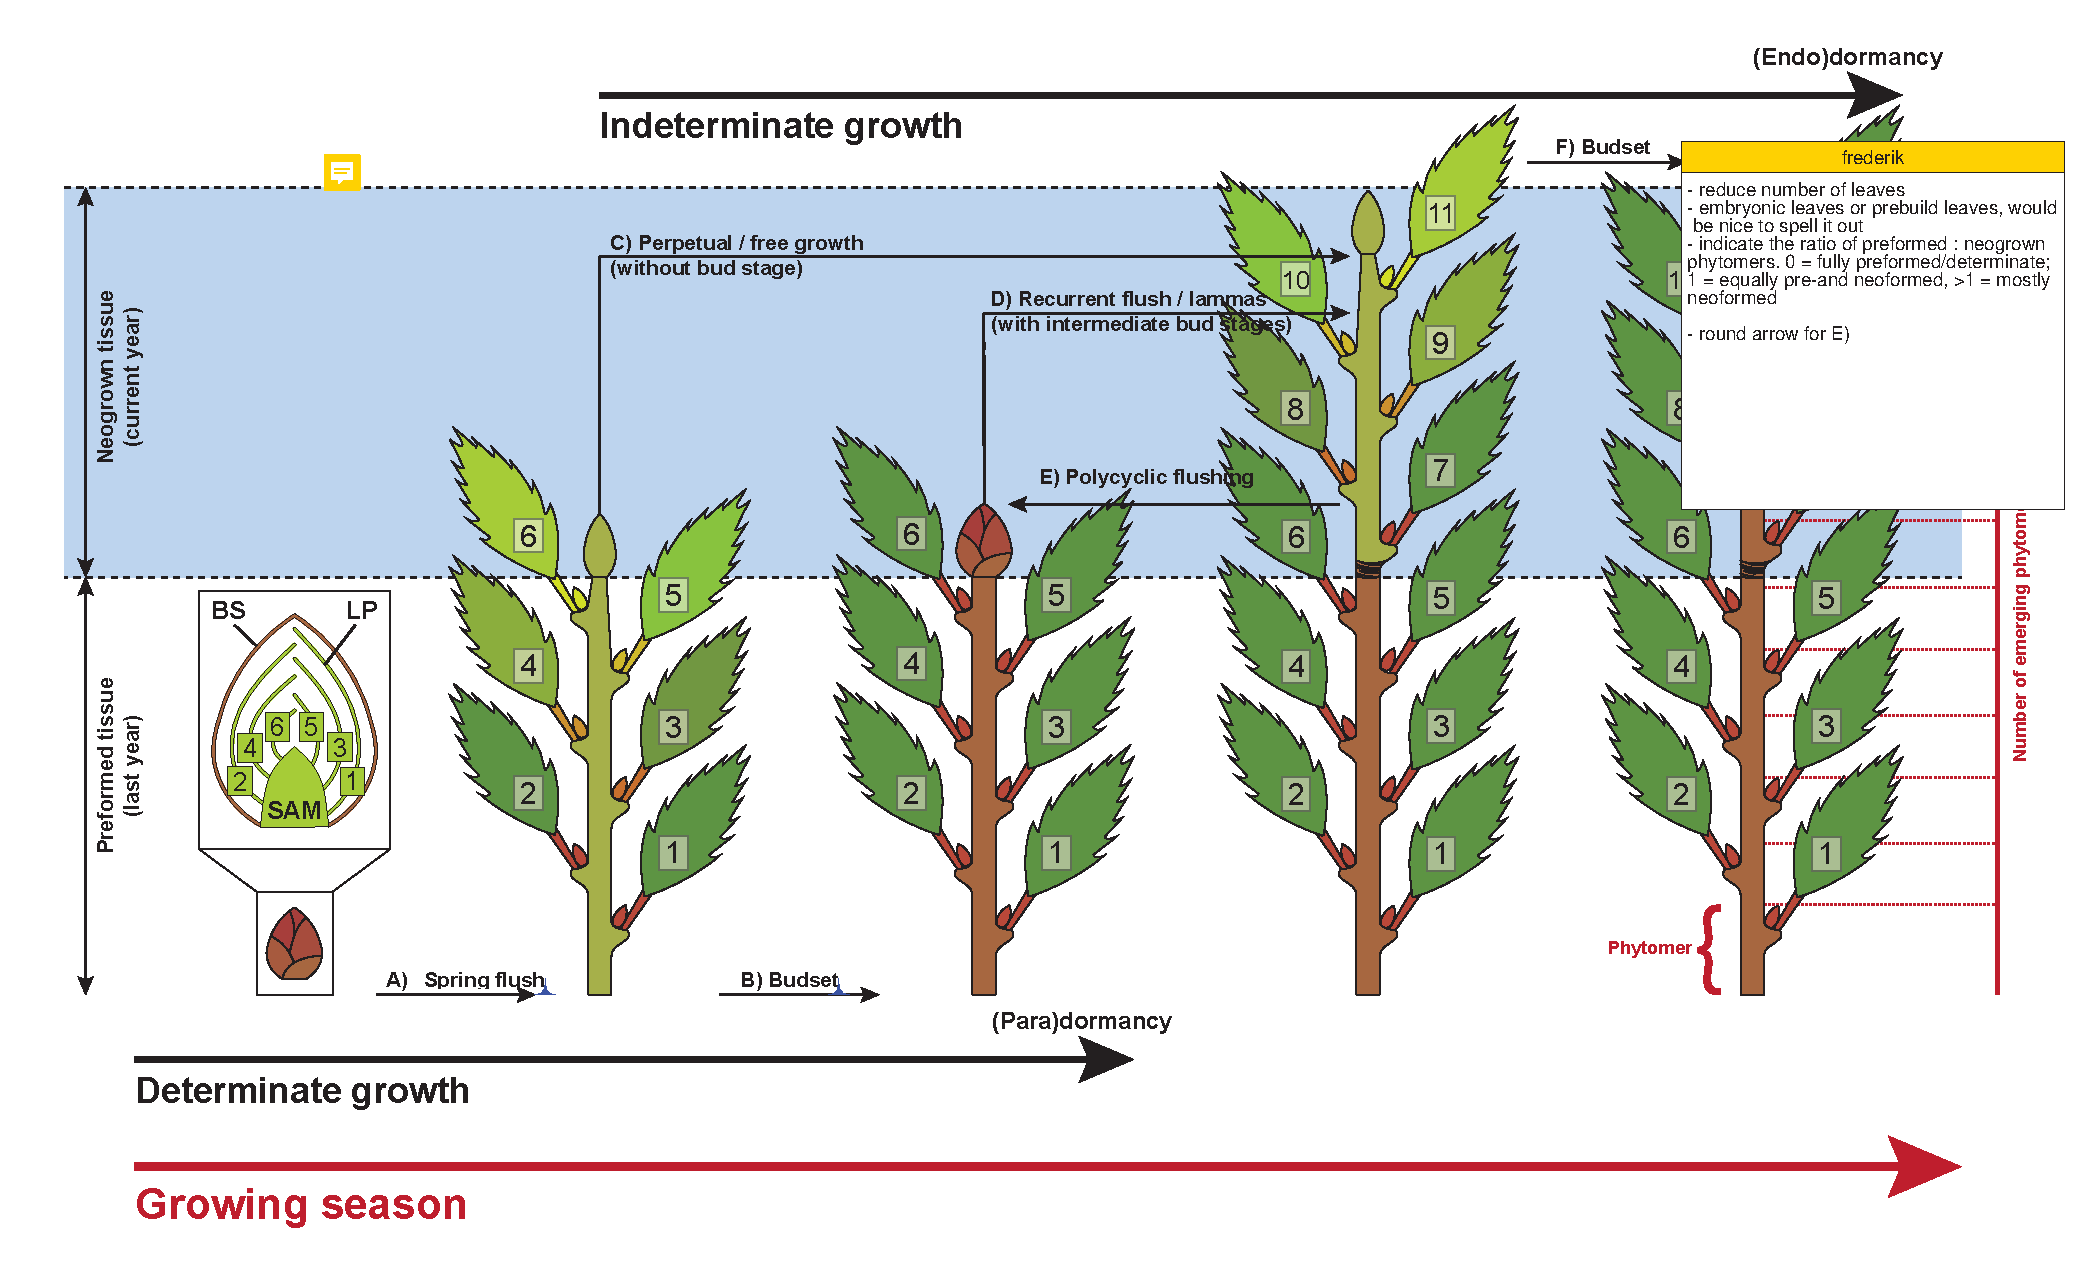
\includegraphics[width=1.1\textwidth]{determinismFigure_FB.pdf} 
								\caption{Determinate and indeterminate growth within one growing season for species producing terminal buds. Commonly all tree species deploy buds during their first (spring) flush from prebuilt and overwintering leaf primordia (A). Determinate growing species set buds (B) that are under hormonal suppression to inhibit any further activity of the shoot apical meristem (paradormancy). Indeterminate growing species continue to produce new phytomers directly (C) or through one (D) to several (E) intermediate bud stage(s). Finally, most species set their terminal buds (F) and enter full dormancy (endodormancy). Shoot apical meristem (SAM); bud scale (BS); leaf primordia (LP). The basic unit of a shoot is the phytomer which is composed of a node, a leaf, the axillary bud and an internode.}
								\label{fig:fig_2xxx}
								\end{figure}
								
	\section*{Control mechanisms of (in)determinacy}
	Despite a century of research into plant growth habits and strategies, we still have a limited understanding of when and why trees exhibit a particular degree of (in)determinacy. This is likely due to the high variability of environmental conditions within and across years, sites, and individuals, which complicates efforts to disentangle internal growth regulation from external environmental influences.
	
	%favourable conditions
	There is indeed evidence that favorable conditions, particularly high soil moisture availability throughout the growing season, can prolong or boost shoot elongation, sometimes enabling an additional flush \citep{kayaAdaptiveSignificanceIntermittent1994}. 
	%root:shoot ratio
	These findings indicate that shoot growth may come to a halt because water supply cannot support expanding leaf area. An imbalance in the root:shoot ratio under a given water status of the plant can indeed suppress shoot growth \citep{borchertSimulationRhythmicTree1973}. By the same mechanism, many species are able to produce new shoots to rebuild the canopy after a considerable loss of leaf area due to herbivory, hail storms or late spring frosts \citep{baumgartenNoRiskNo2023a}.  \\
	
	%provenances, adaptation
	However, environmental conditions do not simply alter a species' growth strategy. While a certain plasticity of apical shoot growth has been shown, this flexibility is often restricted to a specific developmental time window—and is far more limited in determinate species. This reflects a genetically fixed strategy, likely evolved as a safeguard against regular and predictable environmental stress (e.g., frost, drought). In contrast, indeterminate species retain a more open and responsive growth pattern, allowing them to resume or extend growth later in the season when conditions permit. Provenance trials reinforce this idea, showing that the frequency of second flushes is higher in populations from southern origin \citep{rudolphLammasGrowthProlepsis1964, soolanayakanahallyTimingPhotoperiodicCompetency2013a}.\\
	
	%photoperiod
	Latitudinal variation in the frequency of second flushes suggests a photoperiodic regulation comparable to that of bud set in poplar species  \citep{soolanayakanahallyTimingPhotoperiodicCompetency2013a}. Indeed, bud set, growth cessation, and flowering induction appear to be regulated by a shared set of genes (\textit{CONSTANS} and \textit{FLOWERING LOCUS T}) regulated by photoperiod \citep{bohleniusCOFTRegulatory2006a}. Moreover, \citet{wangPlantsDistinguishDifferent2024b} found that plants distinguish between absolute and photosynthetically relevant photoperiods to independently regulate flowering and vegetative growth.  \\
	
	Although photoperiod appears to be a key regulator of seasonal growth and development in many species, most of our knowledge comes from model organisms, with poplar being the prime woody perennial that is extensively studied. Thus, genetic control mechanisms of (in)determinacy that set the potential of tree growth across species are yet to be discovered. \\
	
	%ontogeny as another control mechanism: becoming more conservative and determinate with age	
	
										
	\subsection*{Evolution of (In)determinacy}
	Understanding how universally tissues within species are formed determinately or indeterminately could provide insight into the evolution of this trait, which could be aided by cross-species analyses. Both growth forms seem to occur across most species of the same genera or clade and hence, appear to have evolved repeatedly in different groups (Figure \ref{fig:fig_4xxx}), making it difficult to speculate on which strategy is ancestral \citep[but see][]{hariharanIndeterminateGrowthCould2016} and how rapidly (in)determinacy can evolve. As data on which species are determinate or indeterminate accumulates, such analyses could potentially provide rapid insights into this, and also aid forecasting for unsampled species. Assigning species as determinate or indeterminate, however, may not be useful if the trait is actually continuous. \\

	But what are the fundamental trade-offs associated with adopting either strategy? In most temperate and boreal ecosystems both growth strategies are successful and co-occur, suggesting ecological niche separation. The enhanced growth potential of indeterminate species allows them to easily outgrow competing species. Faster growth, however, might lead as well to higher turnovers and shorter life spans \citep{brienenForestCarbonSink2020b, milletRelationshipArchitectureSuccessional1999}. Not surprisingly, indeterminate growing species are often found to be early successional ones \citep{marksRelationExtensionGrowth1975, boojhGrowthStrategyTrees1982}.
	%section from Sally:
	Moreover, indeterminate growth allows for greater phenotypic plasticity, as tissue is produced in real-time in response to current conditions. In contrast, determinate species preform tissues in advance and are thus more constrained by past conditions, particularly those experienced during bud formation. As a result, determinate species may exhibit stronger local adaptation and reduced short-term plasticity compared to indeterminate species  \citep{leitesForestTreeSpecies2023}. For example, western larch (\textit{Larix occidentalis}) achieves much of its primary shoot growth from indeterminate growth %(a combination of lammas and neoformed shoot growth), 
	and is less locally adapted than the sympatric species Douglas-fir, which grows more determinately \citep{roskillyWeakLocalAdaptation2024}.\\

%As the climate continues to change, the central question becomes: Which growth strategy will prove more successful in the future?

								
%	\begin{mytextbox}[]
	%	\subsection*{Box 1: Definitions)}
	%	\textbf{Growth habit}: The genetic tendency of a plant to form a characteristic habitus (shape, height, form) with a particular branching and growth pattern. \\
%		\textbf{determinate growth}: a growth pattern characterized to stop at a predefined size. Commonly, the apical bud culminates in an inflorescence, halting the production of any additional leaves or buds. In trees this terms specifies the short duration of extension growth in spring with no further activity of the apical meristem.\\
		%\textbf{indeterminate growth}: a growth pattern characterized by continuous growth (leaves, buds or flowers) throughout their life or as long as condition remain favourable. This is possible because the apical meristems always remain vegetative and flowers are restricted to lateral meristems. In trees this refers to the continuous shoot elongation throughout the growing season.\\
		%\textbf{Neogrowth}: Growth that occurs on top of preformed tissue due to the more or less continuous activity of the shoot apical meristem. Several forms occur depending on whether growth occurs continuously or in bursts.\\
		%\textbf{Perpetual/Continuous/free/sustained growth}: the constant production of new tissue without interruptions of bud stages.\\
		%\textbf{Polycyclic flushing:} successive bursts of shoot growth interrupted by bud set and a resting phase within the same vegetative period   \\
		%\textbf{Second flush:} Growth form of species in which one additional cohort of buds is build and deployed during the current growing season. In the German literature this is often termed ‘Johannitrieb’ since the flush often occurs around the summer solstice. Also ‘lammas growth’ is a common term for an additional flush.\\
		%prolepsis = a rhythmic branching process, during which a bud underwent a dormancy phase and subsequently extends into a branch. Determinate species have only proleptic branches.
		%syllepsis = a continuous branching process, during which an incomplete axillary bud without a resting phase extends into a branch. Indeterminate species have both proleptic and sylleptic branches. 
	%\end{mytextbox}

	
\section*{The performance of (in)determinacy with climate change} 

Spring warming has advanced the onset of leaf emergence by up to a month compared to pre-industrial times \citep{vitasseGreatAccelerationPlant2022b}. In contrast, autumn phenology of growth and leaf senescence has not shifted as much as one might expect, given the extension of favorable growing conditions  \citep{zaniIncreasedGrowingseasonProductivity2020b, zohnerEffectClimateWarming2023}. In fact, phenological sequences are increasingly observed to shift as a whole toward spring, rather than stretching at both ends of the growing season \citep{keenanTimingAutumnSenescence2015b, mengConsistentTimeAllocation2024}, not necessarily leading to increased biomass production during longer growing seasons \citep{zaniIncreasedGrowingseasonProductivity2020b}. We hypothesize that determinate species will largely maintain their fixed growth schedules under climate warming, with no or little reductions in overall productivity, due to increased drought and heat stress with little ability to compensate. In contrast, indeterminate species are capable of extending their growth into both spring and autumn, potentially resulting in higher productivity under future climatic conditions (Figure \ref{fig:fig_4xxx}). \\
%Yann: But we should keep in mind that if indeterminate growth strategies is mainly found in early successional species, climate change will not really change the cards, perhaps just accelerate the transition phase between early and late successional species…

However, the greater flexibility of indeterminate species could also increase their exposure to extreme climatic events. Deciduous indeterminate species are often among the first to leaf-out and among the last to shed their leaves---occasionally as a result of first freezing events in autumn. In addition, a substantial part of their growth period falls into periods of summer with increased risk of drought (Figure \ref{fig:fig_4xxx}). 
Therefore, we hypothesize that the conservative strategy of determinate growth largely escapes unfavorable growing conditions by growing between the last spring frost and the increasing water shortages in summer, with relatively ample safety margins in contrast to indeterminate species. Consequently, productivity shows little variation from year to year and will largely remain constant in a future climate or even decline due to higher water stress during their restricted window of potential growth.
However, once hit by an extreme event that damages leaves, determinate species might not recover easily. Even if leaves are shed to prevent further damage, e.g., in response to drought, the loss of the canopy, which is rarely replaced after the summer in determinate species, will prevent replenishment of the reserve pools and ultimately reduce fitness. In contrast, the flexible growth schedule of indeterminately growing species may allow plants to: 1) produce tissue better adapted to harsh environmental conditions as it is formed in the current season (e.g., smaller leaves with higher specific leaf area), and 2) catch up and compensate later in the season by another productivity boost. Taking advantage of a `second growing season' after summer drought was indeed shown for pines in the Mediterranean` climate through polycyclic flushing---a form of indeterminate growth \citep[Figure \ref{fig:fig_2xxx}]{girardPolycyclismFundamentalTree2011}. \\

We argue that new opportunities and challenges for trees with climate change will increasingly disrupt their phenological cycles, favoring species and genotypes that are more plastic in rearranging their activities by resuming growth, reproduction and/or storage restoration (e.g., starch, nutrients) later in the year, thereby recovering from and compensating for some stress-induced damages and losses. Future climate will therefore likely intensify the competition among co-occurring species and might re-assemble forest communities increasingly composed of species adopting an indeterminate growth strategy.
	
	
								\begin{figure}
								\centering
								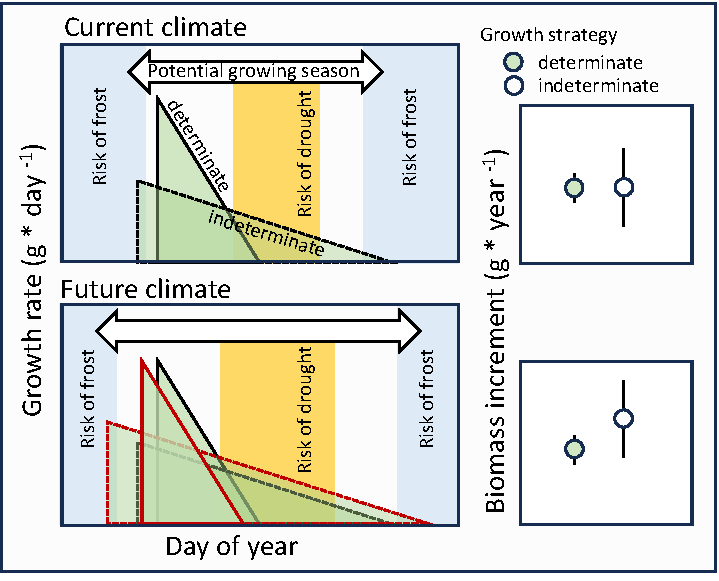
\includegraphics[width=0.9\textwidth]{Fig_3_V4.pdf} 
								\caption{Hypothesized predictions of growth rates under current (upper panels) and future (lower panels) climate for determinate and indeterminate growing species. Note that the indeterminate strategy is more exposed to the risk of frost and drought events while the determinate strategy condenses most growth within a safe period. In the current climate the indeterminate strategy is in balance with benefiting from the full climatic growing season in some years with some drawbacks in other years, resulting in the same mean yearly biomass increment, but with a higher variation; right box). In a future climate the indeterminate strategy might benefit from longer growing seasons, resulting in an overall higher mean annual biomass increment compared to determinate growers, but this will be dependent on the severity of drought that overlaps the potential growth period of determinate species. Triangle outlines represent the activity window for a current (black) versus a future (red) climate.}
								\label{fig:fig_4xxx}
							\end{figure}
	\pagebreak
	
	\subsection*{(In)determinacy beyond leaf tissue} 
	Although (in)determinate growth is typically discussed in the context of the shoot apical meristem, similar patterns may exist in secondary growth and below-ground meristems. For example, in the vascular cambium, a timely transition from earlywood to latewood production---and from vegetative growth to reproductive or storage allocation---may reflect an internal growth schedule similar to that of primary shoot growth. Cambial initial cells divide to form daughter cells, which subsequently produce cohorts of precursors that then mature into functional xylem and phloem \citep{valdovinos-ayalaSeasonalPatternsIncreases2022}. Hence the number of initial cell divisions largely determines the amount of total xylem formed over the season \citep{lupiXylemPhenologyWood2010}. Interestingly, several studies report that wood formation often ceases even when environmental conditions remain favorable and the canopy is still photosynthetically active—suggesting that internal controls may limit secondary growth regardless of external potential  \citep{buttoComparingCellDynamics2020, arendStemGrowthPhenology2024}.\\
	
	Regarding below-ground meristems, roots seem to follow a much more opportunistic and indeterminate strategy with root meristems remaining active throughout the year. Experimental evidence from rhizotron studies even show root growth during mid-winter whenever soil temperatures are suitable \citep{lyfordControlledGrowthForest1966}, suggesting that roots do not enter true dormancy \citep{radvilleRootPhenologyChanging2016, marchandNoWinterHalt2025}. However, the degree to which asynchrony between above- and below-ground meristems reflects environmental conditions (e.g., soil temperature), root:shoot imbalances, or genetically fixed strategies remains unresolved \citep{abramoffAreBelowgroundPhenology2015, makotoSynchronousAsynchronousRoot2020, silvestroRootsLeavesTree2025, campioliEnvironmentalSensitivityImpact2024}.\\
	
	
	%Sally:
	%Seems like there should be a paragraph about deciduous versus evergreen species, and the potential differences in outcomes of (in)determinacy. Of course, evergreen species are not as reliant on the new leaf area produced in a single year – would that lead to a prediction of greater determinacy?
	
	%	\begin{figure}
		%	\centering
		%	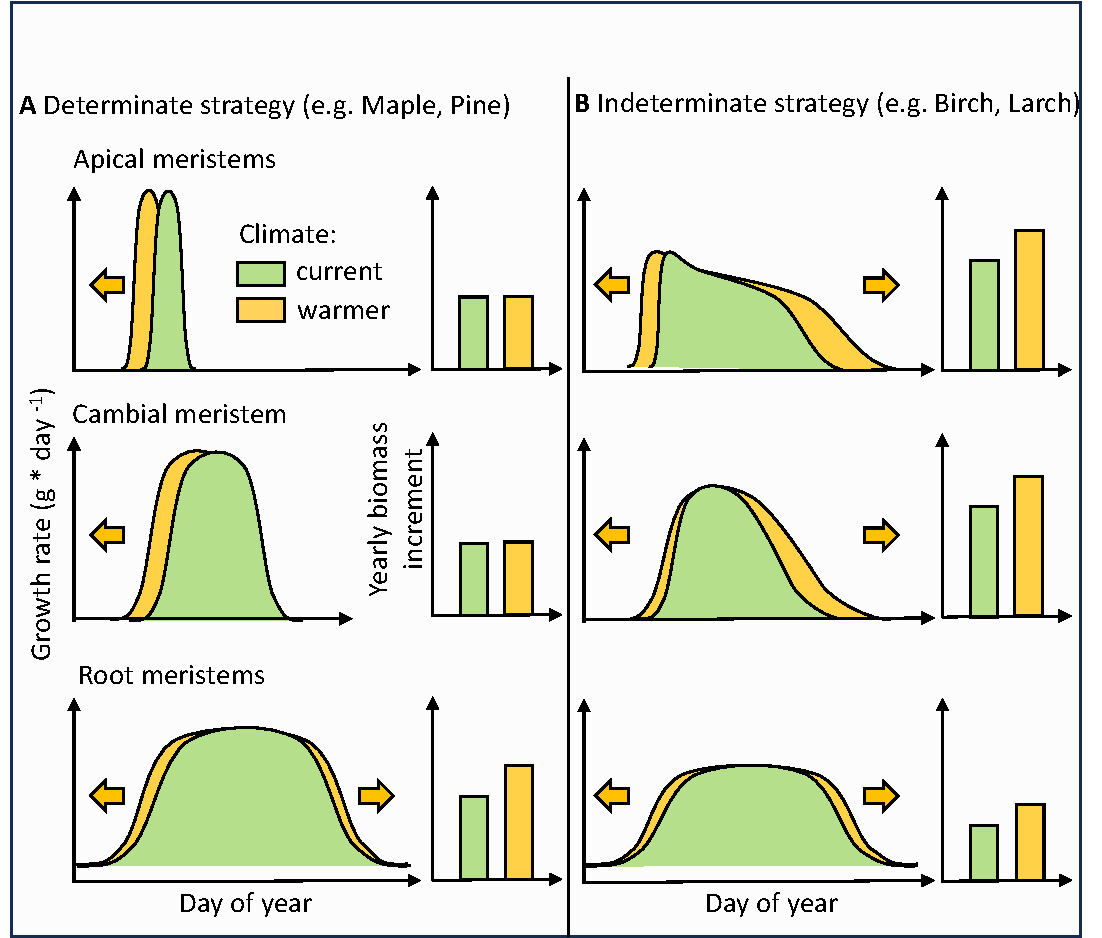
\includegraphics[width=0.9\textwidth]{Fig_3_V3.pdf} 
		%	\caption{Hypothesized predictions of growth rates for the three major meristem (apical, cambium and root) classes of trees under current and warmer climates following an extreme determinate (A) and indeterminate (B) growth strategy. The area under the curve is summarized as yearly biomass increment in the respective bar-plot. Arrows indicate the shift of growth phenology under warmer climate conditions. Root meristems appear to be purely temperature opportunistic for both strategies, even growing during warm winter spells. The indicated genera were observed to showcase the illustrated trends. The responses of these two contrasting growth strategies might apply not only to different tree species but also within a population (e.g. along environmental gradients) and even within an individual as it transitions from the juvenile to the adult stage (ontogeny).}
		%	\label{fig:fig_3xxx}
		%	\end{figure}
	
	\begin{tcolorbox}[
		colback=gray!5!white,  % Background color of the box
		colframe=black,      % Frame color
		coltitle=white,      % Title (header) text color
		fonttitle=\bfseries, % Makes the title bold
		boxrule=0.5pt,       % Frame line thickness
		title=\textbf{Box 1: Metrics of (In)determinacy}
		]
	
		To advance our understanding of growth strategies under climate change, we need improved methods for quantifying the degree of (in)determinacy—moving beyond a simple binary classification. We propose a set of metrics, ranging from organ-level traits to landscape-scale proxies:\\
		

			\textbf{Ratio of preformed to neoformed organs:} 
			The ratio of the number of leaves (or leaf scars) at the end of the season to the number of leaf primordia initially formed in buds provides a direct measure of (in)determinacy. Values greater than one indicate a higher degree of indeterminate growth. First described over a century ago \citep{mooreStudyWinterBuds1909}, this metric has been used in only a few studies \citep{damascosBudCompositionBranching2005, kikuzawaLeafSurvivalWoody1983, guedonRelativeExtentsPreformation2006}. Although quite distinct and easily counted in some species (e.g. maples; \citealt{critchfieldShootGrowthHeterophylly1971}), there are only slight morphological differences between neoformed and preformed leaves in others (e.g., black cottonwood). Time-lapse imaging, labeling or artificial wounding can facilitate the distinction between preformed and neoformed organs. The number of leaf primordia can be determined through bud dissection, but this precludes the counting of neoformed leaves that would later arise from the same meristem. Micro-CT imaging may offer a modern, non-destructive alternative to bud dissection \citep{kovaleskiXrayPhaseContrast2019}.\\
			
			 \textbf{Seasonal growth patterns:} Temporal tracking of shoot elongation and wood formation—via micro-coring, dendrometers, or regular shoot measurements—reveals when and how new tissue is produced. Wood anatomical analyses distinguish cell formation from later development, especially useful in combination with artificial wounding of the cambium that acts as a `marker in time’ (pinning technique; \citealt{gartnerCambialActivityMoringa2021a}). High-resolution LiDAR and photogrammetry are increasingly capable of capturing shoot elongation and structural changes across whole crowns or stands \citep{zhangForestsGrowthMonitoring2019, jinEstimationLarchGrowth2022}.\\
			
			\textbf{Seasonal trends in canopy greenness:} Satellite and drone imagery can track vegetation green-up and senescence at large spatial scales. For example, \citet{mengConsistentTimeAllocation2024} found that time allocation between green-up and senescence remained consistent across temperate ecosystems, despite substantial variation in growing season length and warming intensity.\\
			
		%	\textbf{Ecosystem-scale carbon fluxes:} Eddy covariance towers measure net carbon exchange, providing ecosystem-level signals of growth activity. Extended or bimodal periods of CO$_2$ uptake may reflect indeterminate growth, while sharp, narrow peaks may suggest determinate growth. When combined with phenological observations (e.g., LAI, phenocams), EC data can help infer growth timing and seasonal flexibility.

	\end{tcolorbox}
	
	
\section*{Future directions}
We argue that incorporating plant determinacy into models of forest dynamics could greatly improve predictions of how climate change will affect ecosystem composition and productivity. The impacts of both climatic extremes and longer growing seasons on primary and secondary growth may depend strongly on the relative abundance of determinate versus indeterminate species within a forest community. Better understanding these two strategies and their response to a warmer and a drier climate will help to reveal the potentials and limits of trees to adapt in a future climate, and may inform species or provenance choices in forest management.

One critical knowledge gap lies in understanding how different degrees of (in)determinacy help trees avoid or buffer environmental stress, while still maintaining the capacity to resume growth, repair tissues, replenish reserves, and compensate for earlier losses within the same season. Clarifying the trade-off between escaping unfavorable conditions and exploiting longer growing seasons is key to anticipating how forest communities will respond and reassemble over the coming decades.\\

Moving forward, we need to characterize the plasticity of indeterminate growth across environmental gradients, species and populations with a particular focus on how much they are under genetic control. 
This will require integrative research combining genetics, physiology, ecology, and phenology. Moreover, we must assess how the prevalence of indeterminate growth affects forest-scale carbon dynamics, especially if (in)determinacy proves to be a continuous trait rather than a binary one. 

Finally, we need to link the temporal dynamics of primary (apical and root) and secondary (cambial) meristems. Correlating annual tree rings with shoot increments could reveal such a common pattern, provided that the timing of inter-annual shoot segment (phytomer) production is accounted for, e.g. by distinguishing between phytomers that are preformed and those that are neoformed. Revealing the patterns of when different meristems are active will likely contribute to a theoretical framework of temporal carbon allocation dynamics, and thus ultimately improve predictions on future forest carbon sequestration.


	

	%

	
\section*{Acknowledgments}
	This text emerged from a grant of the Swiss National Foundation to F.B. (grant number P500PB\textunderscore 210943). We thank J. Ngo for designing figure 2.
	
	
	\pagebreak
	

	\newpage
%\section*{stuff I did't find place yet}

%Deciduous tree species have a higher number of leaf primordia inside their buds than evergreen species in the Cerrado (Brazil). 
	
%If experiments are conducted in conditions with unlimited soil moisture and under similar temperature regimes, then the dynamics of growth responses can be comparable among species and reveal their potential in deploying indeterminate growth. Under natural conditions with common soil moisture and associated turgor limitations it is currently hard to tell if trees cease growth because of a response to the environment or because of switches in resource allocation. 
 
% Even in grasslands an earlier onset of growth is associated with an earlier stop under climate warming \cite{mohlGrowthAlpineGrassland2022a}
	
	
%	must include: 
	
%	\cite{iwasaOptimalGrowthSchedule1989}
	
	
	
%	Shoot growth patterns do not only tell us something about the plant architecture and the strategy of space exploitation, but may reveal also patterns of the whole-plant dynamic and potential of growth and carbon sequestration.
	
%	unit of extension vs. unit of morphogenesis: Perhaps state somewhere that we commonly only observe the extension pattern while patterns of organogenesis remain hidden. 
	
%	\citep{verduEvolutionaryCorrelationsPolycyclic2007}: polycylcic flushing in acer might be associated to maximize the light capture in the understory
%	ontogenetic changes towards monocyclic growth might reflect the urge for light in the early life phase
	
%	 \citep{wuPhenotypicPlasticitySylleptic2001}: proleptic and sylleptic branching. great reference for phenotypic plasticity and how sylleptic growth (a form of indeterminate growth) might be beneficial more stressful/unpredictable climates
	
%	\citep{moreno-cortesCsRAV1InducesSylleptic2012}: Chestnut CsRAV1 is a gene that is under circadian control and induces sylleptic branching when over-expressed in hybrid poplar. Its a promising candidate to enhance biomass production in trans-genic plants. It is intriguing that genes are identified and suggested to be used in trans-genic plants to enhance biomass production, but at the same time we even don't know if there is a correlation of sylleptic branching and biomass production among forest tree species.
	
%	\citep{hollenderMolecularBasisAngiosperm2015} recent review on architecture
	
%	\citep{wuQuantitativeGeneticsGrowth1998}Quantitative genetics of growth and development in Populus. III. Phenotypic plasticity of crown structure and function
	
	\newpage
	
	\bibliography{refs_determinism}
	\bibliographystyle{ecolett}
	
	
	
\end{document}






